\chapter{State of the Art} \label{chap:State of the Art}
% introduction

\section{Implementation of Reactive Systems}
	\subsection{Reactive Programming}
	%"Reactive programming provides dedicated language abstractions for reactive software. Reactive programming relieves developers from manually updating outputs when the inputs of a computation change, it overcomes a number of well-know issues of the Observer design pattern, and it makes programs more comprehensible." [github, rxScala guido] Its also declarative instead of imperative.
	% reactive programming is in general not asynchroneous but it can be used in async context.? (waqas says something different for RXjs)
	% observables, difference to Observer design pattern:
		% observables in a reactive system return/provide multiple values (a stream) instead of just the current state.
		% "Observables provide abstractions over a stream of events. Promises are synchronous executables with a single return value, whereas observables are asynchronous executables that return multiple values over time." [pradeep]
		%"The data produced by the producer is stored in observable which the consumer consumes."[Pradeep]
	% observables are also called signals[wikipedia] = values that vary over continuous time -> or in RxJs Observables, Bacon Properties
	% events = events which have occurrences at discrete points in time -> RxJs Subject, Bacon EventStream
	% "observables" are functions that tie an observer to a producer. A producer creates values over time. An observer reacts to the values of a producer and notifies all subscribers (in a push based system).
	%operators: "Each operator outputs an another observable without modifying the original data streams." [Pradeep]
	% push and pull based: 
		%"Push-based systems take events and push them through a signal network to achieve a result. Pull-based systems wait until the result is demanded, and work backwards through the network to retrieve the value demanded." https://en.wikipedia.org/wiki/Functional_reactive_programming
	% cold and hot observables https://medium.com/@benlesh/hot-vs-cold-observables-f8094ed53339
			% -> author: "RxJS 5+ Lead, Software Engineer at Google, RxWorkshop.com. Own view, not the companies"
		% cold: the subscribe call creates the producer - one producer (e.g. a websocket raising events) is created for each call to subscribe, it gets destroied if the observer unsubscribes -> unicast
		% hot: all calls to subscribe (usally) share one producer - multicast
		% Rx Subjects - functions as both observer and observable, multicast but will terminate if the last subscriber is unsubscribed, can not be reused after termination or if in error state. "It multicasts. All observers passed to it via `subscribe()` are added to an internal observers list."
			% "Armed with our Rx Subject above, we can use a bit of functional programming to make any “cold” observable “hot”:
			%function makeHot(cold) {const subject = new Subject();cold.subscribe(subject); return new Observable((observer) => subject.subscribe(observer));}
			%Our new `makeHot` method will take any cold observable and make it hot by creating a subject that is shared by the resulting observable."
			% in RxJs that is e.g. publish or share
	
	\subsection{RxJs and BaconJs}
	% Though there are other JavaScript implementations of the reactive design pattern like https://github.com/stoeffel/awesome-frp-js,
	% kefir, cyclejs
	% this thesis focuses on RxJs and BaconJs, because these are the one the extension currently supports.
	
	%RXjs
	%var button = document.querySelector('button');
	%Rx.Observable.fromEvent(button, 'click')
	%.throttleTime(1000)
	%.scan(count => count + 1, 0)
	%.subscribe(count => console.log(`Clicked ${count} times`));
	% - The essential concepts in RxJS which solve async event management are:
	%Observable: represents the idea of an invokable collection of future values or events.
	%Observer: is a collection of callbacks that knows how to listen to values delivered by the Observable.
	%Subscription: represents the execution of an Observable, is primarily useful for cancelling the execution.
	%Operators: are pure functions that enable a functional programming style of dealing with collections with operations like map, filter, concat, flatMap, etc. Each operator output another observable without modifying the originial data stream.
	%Subject: is the equivalent to an EventEmitter, and the only way of multicasting a value or event to multiple Observers.
	%Schedulers: are centralized dispatchers to control concurrency, allowing us to coordinate when computation happens on e.g. setTimeout or requestAnimationFrame or others.
	% - "The subscribers are not locked in a synchronous request and there can be an infinite sequence of next emissions from the observables to the observer." [Pradeep] although subscribing is in general a synchroneous operation.
	% - "completed and error functions	being defined at the observer, which are invoked by the observable on respective events. This lets the observer know that an observable has exhausted sending values, or an error has occurred	when performing an operation on the observable." [Pradeep]
	% - "Subjects can be both observable and an observer[37]. It is a special type of observable which	allows values to be multicasted to many observers" [Pradeep]
	% - "Unsubscribing is an optional feature in RxJS as RxJS handles this by default but it makes sense to unsubscribe manually by a user if the source observable is emitting the values continuously and the user does not need values after a specific point of time." [Pradeep]
	% - "With the support of RxJS, we can convert multiple values, arrays, events into observables."[Pradeep]
	% - current version in development 6.0.0-alpha.2, stable: 5.5.6
	% - github stats 31.1.2018 18:22 for current active version (they changed repositories multiple times): watch: 387 star: 10,540 fork: 991 contributors: 185 but since they changed the repository the total numbers for all versions are much higher.
	% licence: Apache 2.0 latest commit: 30.01.2018
	% first release on github: version 2.2.0 01.03.2013
	
	%Baconjs: 
	%Generally, this is how you implement an app with Bacon.js. Capture input into EventStreams and Properties - Transform and compose signals into ones that describe your domain. - Assign side-effects to signals.
	%EventStreams (distinct events) and Properties (values that change over time). 
	%$("#username input").asEventStream("keyup").map(function(event) { return $(event.target).val() }).toProperty("")
	% "In Bacon, these are two flavors of Observables. EventStreams and Property are two basic concepts	of Bacon.js that are basically known as events and behaviours in the literature of FRP." [waqas]
	% - BaconJS does not have cold observables [ref baconjs github - For RxJs Users]
	% - "Error handling is also a bit different: the Error event does not terminate a stream. So, a stream may contain multiple errors. To me, this makes more sense than always terminating the stream on error; this way the application developer has more direct control over error handling. You can always use stream.endOnError() to get a stream that ends on error!" [baconjs github]
	% - it has the "spy" feature which greatly reduces the required effort to create complementary tooling like CRI or RxFiddle. It can also be used to easily create extensive logging.
	% - created because "Bacon.js exists largely because I got frustrated with RxJs, which is a good library, but at that time didn't have very good documentation and wasn't open-source. Things have improved a lot in the Rx world since that. Yet, there are still compelling reasons to use Bacon.js instead. Like, for instance, more consistent stream/property behavior and (arguably) simplicity of use." [baconjs github]
	% - current version 2.0.0
	% - github stats 31.1.2018 18:22: watch: 156 star: 5,839 fork: 328 contributors: 83
	% licence: MIT latest commit: 30.01.2018
	% -> has a smaller community than RxJs
	% first release on github: version 0.7.90 08.03.2017
	

\subsection{Debugging Reactive Code}
The violation of a syntax rule of in a programming language such as missing control characters, misspelled keywords etc. are syntax errors and can be detected by most IDEs very precisely, but logical errors are harder to track down. Modern IDEs use breakpoints including conditional breakpoints, step by step execution, event logging, stack traces and many more. Due to reactive programming being declarative, breakpoints, the most useful feature for in-depth code and state inspection at a precise point during the applications execution can not be used as easily. For some IDE even chained function call provide a obstacle because there breakpoints are line and not character position based. But even if the IDE can handle breakpoints inside lambda functions for the usual navigation features like \emph{Step Over} and \emph{Step Into} it is not trivial to balance between providing the necessary fine grained stepping and having to many steps for the developer to iterate. For example one of the most advanced IDEs there is, Visual Studio (2017) for .NET, will step over the whole batch of chained functions if the developer uses \emph{Step Over}, but will step into the first lambda function in the chain if the developer uses \emph{Step Into}. The developer can then use \emph{Step Over} to enumerate the lambda functions passed to the chained functions (see listing \ref{lst:CSharp_LINQ}). This is a very specialized and desirable behavior that will match the intend of the developer most times when using the .Net Framework built in \emph{.NET Language-Integrated Query Expressions} (LINQ), but this behavior will break as soon as a custom function is added to the chain (\emph{DoCustom} in the code example). Now the \emph{Step Into} on line 1 will step into \emph{DoCustom} for each entry in the list and will then step out of the batch of chained functions to line 10. If a similar code example in Bacon.js is debugged with the step-by-step debugging feature of Google Chrome, it will actually step through the Bacon.js framework code even if the developer just uses \emph{Step Over}. Because Bacon.js or other reactive programming frameworks are not part of native JavaScript Google Chrome as no means to determine if the user wants to step through the framework code or not.
This example shows that debugging declarative code is still a hard task for modern IDEs, especially if Out-of-Order execution (LINQ Expressions are executed Out-of-Order) is added.
The developers intention is not easy to interpret by the IDE, because there is a multitude of possible steps to take there. The developer could want to debug the custom chained function, they could want to iterate the lambda functions passed as arguments to the chained functions, they could also want to step through the framework functions (Select, Where, OrderBy, etc. which is possible if framework debugging is enabled in Visual Studio 2017 for .NET). 
For big collections, or in the case of reactive programming, observables with many submitted values this problem is also increased by having too many single executions of a lambda function for the developer to step through. Another example for this would be a breakpoint inside a lambda function that is passed to a declarative function (like\emph{Where} in C\# or \emph{map} in Bacon.js) which would halt the application for each element in the collection or data stream.

%TODO: language is c# but the compilation would not complete with "[Sharp]C" as language.
\begin{lstlisting}[language=JavaScript, caption={Simple example of .NET LINQ in C\# to show the steps the visual stidio 2017 for .NET debugger takes while debuggin step-by-step.},label={lst:CSharp_LINQ}]
 var lst = new List<string>{"test1","test2"};
 var result = lst.Select(s => s.ToUpper())
 .Where(s =>
 {
	var b = s.StartsWith("t");
	return !b \&\& s.StartsWith("T");
})
.OrderBy(s => s)
.DoCustom()
.ToList();
\end{lstlisting}


This shows that a traditional debugger is not suitable to use with declarative programming especially reactive programming. While the the Visual Studio debugger is still somewhat useful to debug LINQ in .Net, because multiple specialized behaviors have been implemented over the years and LINQ expressions will most likely not cover the entire application and are often used to execute short tasks inside an imperative program flow, observables in a reactive application are usually much more intertwined and make up the general flow of the program; making a traditional debugger more of an obstacle.

As described in \cite{MSDN_DebugginObservables} reverting to the most basic debugging technique sometimes called \emph{printf-debugging} (or in the Rx.js terms \emph{do-debugging}), to generate debug outputs or traces by directly modifying the source code, generally provides better results than using advanced features of a traditional debugger.
Some of the shortcomings of this basic technique can be mitigated by using sophisticated tools like shown in \cite{ShinyGraphFromLog} in the section "The Reactive Log" where the log of an application is visualized in a dependency graph containing code pieces as nodes, do-debugging still requires the source code to be modified and polluted with statements that do not contribute to the program logic itself.
% requires manual modification of source code to trace program execution.

%- "lack of abstractions" and "mismatch in the mental model" [paper guido1]. "Traditional debuggers are mostly based on runtime stack information and do not consider any other abstraction within the running code." [Abbas]
% - "Missing dependencies are hard to detect with traditional debuggers." [paper guido1 4.1]

The programming language JavaScript (JS) is, unlike compiled languages, harder to debug, because it is an interpreted script language and the JS code is not compiled before execution. The general advantage of being able to change the code during execution and having no compile time, are shadowed by the fact that many bugs can only be found at runtime. 

%...

Currently there are few tools to help the developer debug reactive applications and apart from RxFiddle (described in detail in section \ref{sec:RxFiddle}) non of them, as far as we known, support debugging reactive JavaScript applications. One of those tools is \cite{ShinyGraphFromLog} as mentioned above. Another is the Reactive Inspector for the Scala language \cite{ReactiveInspector} started and maintained by Prof. Dr. Guido Salvaneschi working in the Software Technology Group of the Technical University of Darmstadt, Germany.
The Reactive Inspector is an extension of the Scala IDE for Eclipse. Many features and the basic concepts taht are implemented in the \emph{Chrome Reactive Inspector(CRI)} originate from the Reactive Inspector; including the representation of observables and their dependencies in a dependency graph called \emph{Reactive Tree}, the possibility to query the history of said %TODO can "said" be used?
 graph or the possibility to search for a specific node in the current graph. They are described in details in section \ref{sec:PreviousCRI}. One main feature of the Reactive Inspector, called \emph{Tree Outline} where the user can quickly jump to different areas of the dependency graph, which is useful for applications with large graphs, is currently not implemented for the CRI.

\section{Previous and Related Work}
	\subsection{The Chrome Reactive Inspector}
	\label{sec:PreviousCRI}
		\subsubsection{Master Thesis by Waqas Abbas}
		% main focus of the thesis
			% - proof of concept
			% - how to intercept calls to reactive framework
			% - how to retrieve additional details for each node like the variable name via instrumentation of the source code to give context to observables shown in the dependency graph
		% implemented result of the thesis in short
			% - reactive breakpoints
			% - history queries
			% - Bacon support and partly support for Rx
			% - dependency graph, nodes, edges, zoom, highlighting of current node
			% - instrumentation, dynamically reloading of the page to intercept the JavaScripts for instrumentation
			% - first batch of test applications
			% -> focus on new implementation and prototypes of features and less on maintainability and reliability.
			% -> proof of concept
		
		\subsubsection{Master Thesis by Pradeep Baradur}
		% main focus of the thesis:
			% support for all RxJS operations and RxJS Subjects -> hard to implement, because there is no uniform way like the Bacon.spy method. For details on the general approach see \cite{ThesisBaradur}. For source code see "rx-interception.js"
		% new features introduced:
			% - support for all operations and Subjects in RxJs
			% - loading of some CRI content scripts only when the CRI panel is opened. Istrumentation only when CRI panel is opened.
			% - find dependencys, dependents
			% - added many test applications
			% - improved reliability
			% - less focus on maintainability but move the project further to being usable in a production environment by adding framework feature support.
			% - rearranged UI, changed many styles to defaullt jquery-ui layout.
		
		\subsubsection{Merging previous efforts}
		%- took chrome-reactive-inspector 2 as base and merge all later developed features into it, piece by piece. manually copied changes by Pradeep from Waqas's repository. Hard to detect, changed to match other variable names before committing.
		% - uncompatible git histories - solvable but not much use since the files had separated so much in text character changes, though not so much in logic -> renames and splitting of files
		% - access to many global variables made tracking down dependencies of components hard with mixed contexts - some files with the window object corresponding to contentscripts in the same directory as files with a window object corresponding to the extensions window.
		%TODO: change tone to always present problems as general difficulties instead of shortcomings
		% - merged additional features of Abbas with framework support from Pradeep
		
		\subsubsection{"Special Curicumstances"}
		% demo version of jalangi
		% instrumenting files via scanning the html for script tags
		% -> will not work for module loaders like require.js or ecma6
		% -> will not work with bundled JavaScript code - but since in development there should be a non bundled version available not 
		% a big problem in JavaScript. But for TypeScript since the extension does not support it and when compiling there may already be bundling in place. (#add some text from future here#)
		
		% Shared context through "new Function" that breaks the separation enforced by chrome. To increase consistency and prevent different execution contexts the previous eval was replaced with "new Function" but this does not reduce the security risk.There are other options to execute scripts from a chrome extension but since some of the extension scripts need to share the Rx or Bacon object with the inspected pages JavaScript files there is no other way. ofcorse that breaks the normal isloated world and intodruces a new set of problems like conflicting names. The security risk involved in executing a foreign script in a "trusted" extension context could be reduced if a sandbox was used as described in https://developer.chrome.com/extensions/sandboxingEval. Then all the inspected pages content scripts and some special recording scripts could be executed in that sandbox and transmitt the recorded nodes back via message passing.
		% - Dangers of using eval -> execution in current context. if called from other function, "this" might change. Function() for global with window passed to execute in original context.
		%- Note that  files that are not selected for instrumentation will still generate nodes in the graph, because the Rx and Bacon frameworks will still record interactions, just the information provided by instrumentation is missing.
		%- The Bacon and Rx scripts are prevented from loading so the extensions own files can be used. This is accomplished by filtering all referenced js files in the inspected page for any Bacon or Rx library files and excluding them from the loading process. They need to match version exactly though. This is necessary to guarantee that both work with the same Rx/Bacon object.
	

	\subsection{RxFiddle}
	\label{sec:RxFiddle}
	% RxFiddle is the main competitor with CRI since it is the only other tool (that we are aware of) that tackels debugging for reactive JavaScript systems. Currently the only reactive framework that is supported is RxJs.
	% features of RxFiddle
	% limitations: 'one of the limitations of RxFiddle is ... which we tackeld in this work.
		% - requires more setup to use with web sites that have DOM logic and applications with more than one JavaScript files, although it is possible according to the author \cite{RxFiddleTutorials}.
		% - the variable names in the source code are not displayed in the ui. RxFiddle instruments RxJs to collect its data, not the source code itself like CRI.
		% - fast updating observables like "interval" since each value update creates a new marble for the observable, the view becomes encoumbered fast with this type of observables. As of this moment CRI also generates one or more steps for each update (if the node is not explicitly excluded), but it is easier to examine the value of a node in the first or last few steps (jump to the step and use the next/previous button). CRI can also query the result which provide means to cope with large dependency graphs or histories. In RxFiddle the limitating factor for the fine grained stepping is the available space and resulting overplotting of the value-marbles since the examination is implemented via tooltips on mouseover. For performance comparison see \ref{sec:PerformanceEvaluation}.
		% - like the author explained in "https://github.com/hermanbanken/RxFiddle/issues/6" the web app can not work with large applications properly. The displaying of large applications in one graph is hard for both tools \ref{sec:RapidlyUpdatedObservables}, but RxFiddle needs more spaces for a single reactive operator than CRI. A large dependency graph with descriptive nodes is easier to examine than a large marble diagram that only shows information on nodes in tooltips except in the details view of a currently selected node so finding the desired node/operation is not as easy. RxFiddle also has performacne issue while rendering huge diagrams according to the author. RxFiddle would porbably need another view to appropiately cope with such large applications to help the user navigate and give an overview, although for mid-sized applications the graph on the left side where a user can choose which operation to examine can serve this purpose - As mentioned earlier RxFiddle does not porvide variable names which may lead to confusion of nodes if similar observables are in the same application.
		% As of now, CRI does not support multiple variables having the same name. The author describes some other options like priority ranking in the GitHub issues for the RxFiddle repository \cite[Issues]{RxFiddleGitHub}.
		% - as mentioned erlier RxFiddle onyl supports RxJs while CRI also supports Bacon.js
	% - The author plans to support multiple collectors in the future for web applications, RxScala, RxJava, RxSwift and/or RxNet (source: "https://rxfiddle.net/tutorials.html#attached") which would provide the necessary data collection on one of these platforms and transmit this data to the RxFiddle tool/web-application to be able to use the same debugging environment (RxFiddle) with any of these platforms.



% end of state of the art chapter
%----------------------------------------------------------------------------
%latex sample code:



%\begin{figure}[!h]
%	\centering
%	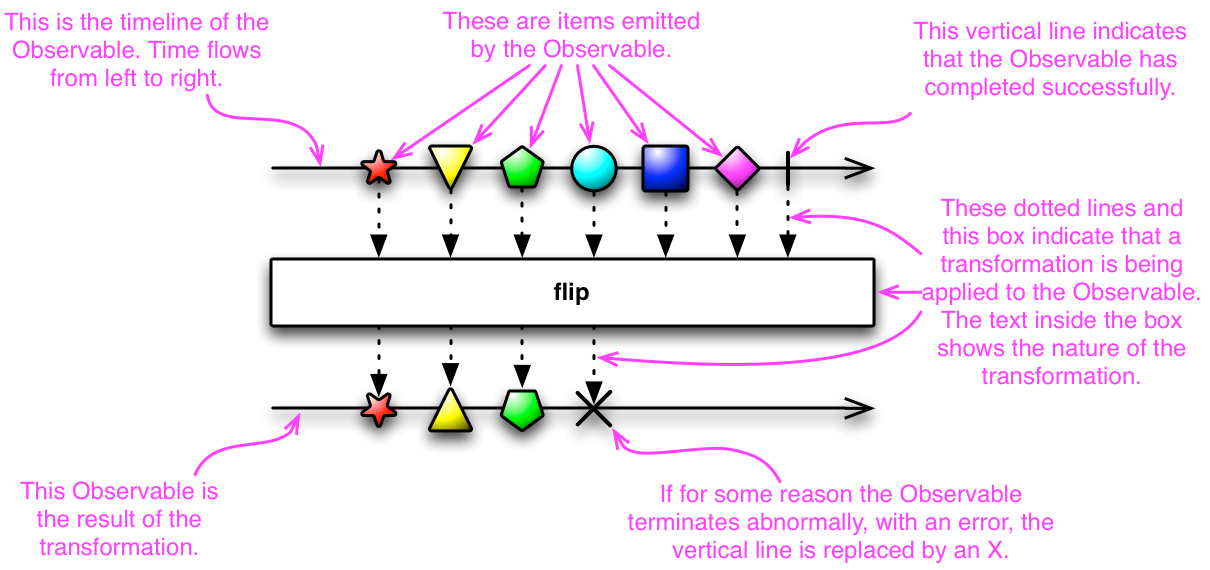
\includegraphics[scale=0.5,trim=0 0 0 0]{gfx/rxjs-reactive-pattern2.png}
%	\caption{Reactive pattern \protect\cite{ReactiveXobservable}}
%	\label{fig:rxjs-reactive-pattern}
%\end{figure}

\textbf{Observable and Observer}\\
Placeholder

\textbf{Operators}
\label{subsec:Operators}\\

\textbf{RxJS Code Structure}\\
Placeholder
\begin{lstlisting}[language=JavaScript, caption=RxJS Simple Example, label={lst:RxJS_Simple_Example}]
// 1. Srouce Observable Creation
var sourceObservable = Rx.Observable.interval(1000);
// 2. Transformation by applying different operators
var transformedObservable = sourceObservable.map(function(x) {
		return x * 10;
	})
	.filter(function(x) {
		return x !== 20
	})
// OUTPUT
Next: 0
Next: 10
Next: 30
Next: 40
Next: 50
Completed
\end{lstlisting}

\subsection{Bacon.js}

\textbf{EventStream and Property}\\
Placeholder

